\chapter{\babSatu}



\section{Latar Belakang}\label{latar-belakang}

Program Enrichment merupakan bagian dari kurikulum Universitas XYZ yang memberi mahasiswa pengalaman pembelajaran berbasis praktik. Program ini terbagi ke dalam beberapa jalur, dan penelitian ini difokuskan pada jalur magang (\textit{internship}). Selama menjalani jalur magang, setiap mahasiswa didampingi oleh seorang Faculty Supervisor yang bertugas memberikan arahan akademik, memantau perkembangan, serta mengevaluasi mahasiswa sepanjang periode program. Karena pendampingan ini memengaruhi capaian pembelajaran mahasiswa, kesesuaian bidang keahlian antara mahasiswa dan Faculty Supervisor menjadi pertimbangan yang menentukan mutu bimbingan.

Penugasan Faculty Supervisor saat ini masih ditangani secara manual. Berdasarkan wawancara terstruktur bersama Margareth Setiawan, Yulianto, dan Mila Andria Savitri selaku \textit{Enrichment Program Coordinator} (EPC) dari tiga fakultas di XYZ University pada 13 Desember 2025, pemetaan mahasiswa ke Faculty Supervisor dikerjakan menggunakan \textit{spreadsheet}. Untuk satu \textit{batch} yang dapat mencapai ratusan mahasiswa, proses ini memakan waktu satu hingga tiga minggu dan kerap disertai revisi berulang hingga dua puluh kali per \textit{batch} akibat kesalahan penempatan. Penetapan pembimbing pun cenderung dilakukan tanpa mempertimbangkan kesesuaian bidang keahlian, sehingga sebagian mahasiswa memperoleh Faculty Supervisor yang kurang relevan dengan topik magangnya.

Cara kerja manual ini membawa beberapa akibat. Beban bimbingan antardosen menjadi tidak merata karena tidak ada acuan kuota, sebagian mahasiswa ditempatkan di luar bidang keahlian pembimbingnya, dan setiap kesalahan penempatan menuntut EPC menyunting ulang data secara manual. Hal-hal tersebut menambah beban kerja EPC dan menyulitkan penelusuran alasan di balik setiap penempatan.

\begin{figure}[h]
\centering
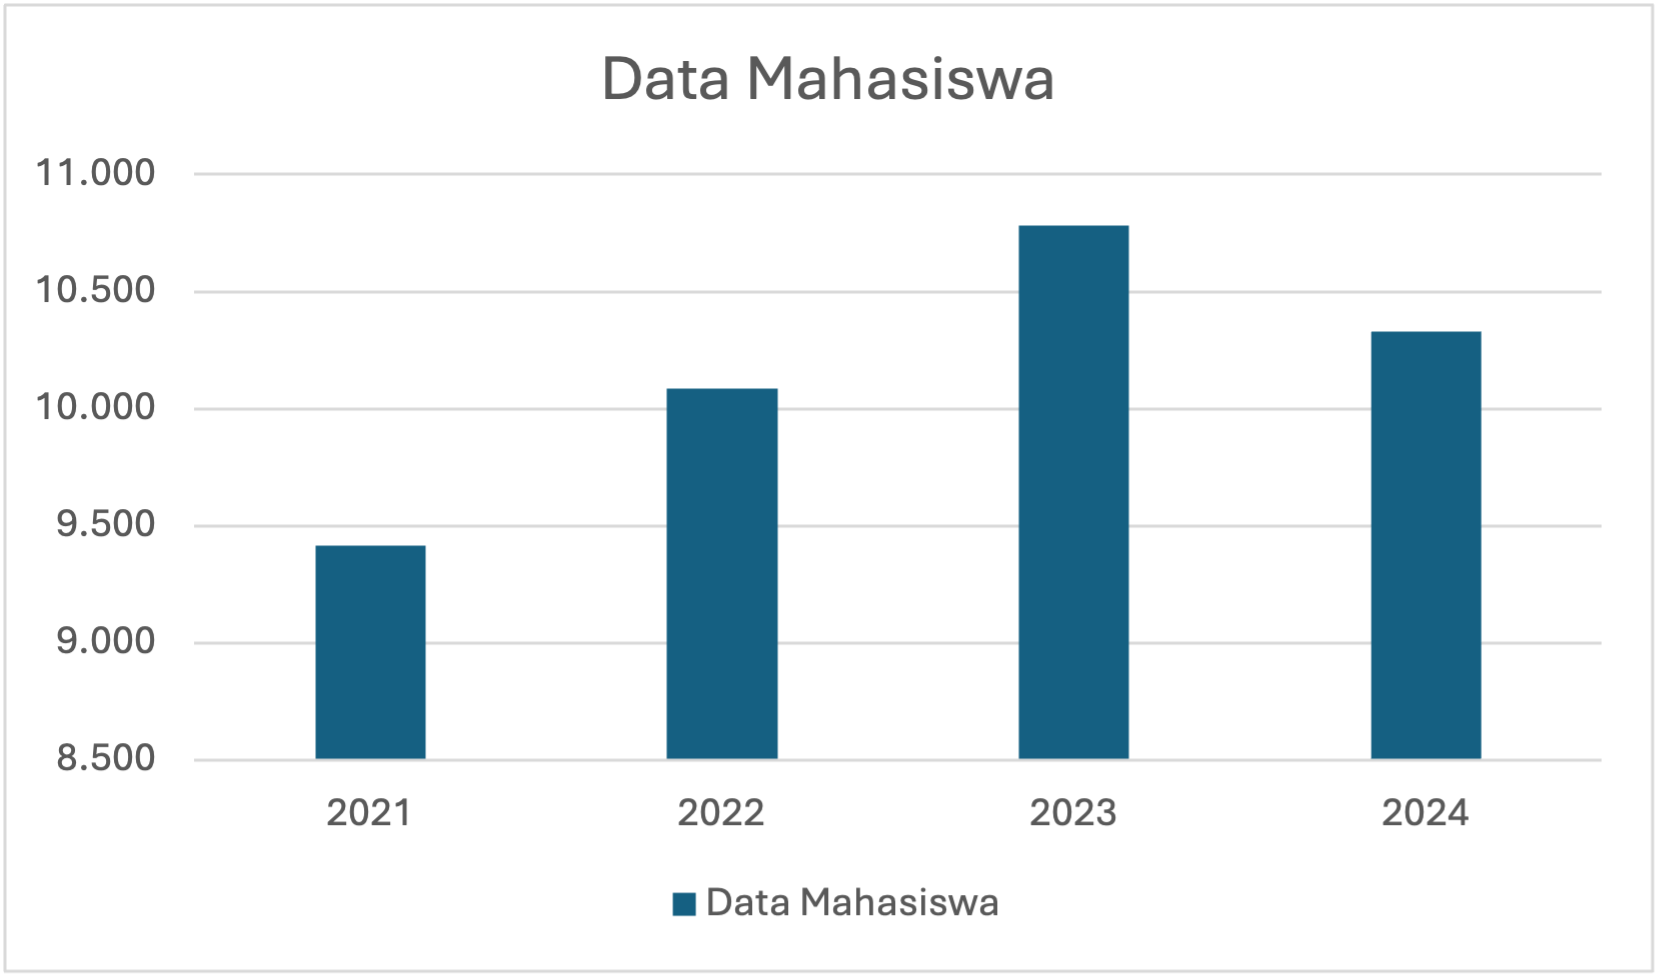
\includegraphics[width=0.85\linewidth]{pic/pertumbuhan-mahasiswa}
\caption{Pertumbuhan Jumlah Mahasiswa XYZ University Tahun 2021--2025}
\label{fig:fig1.1}
% {\footnotesize Sumber: Diolah dari \cite{binusmaba2021}, \cite{binusmaba2022}, \cite{binusmaba2023}, \cite{binusmaba2024}, \cite{binusmaba2025}}
\end{figure}

Beban proses ini bertambah seiring meningkatnya jumlah mahasiswa XYZ University pada periode 2021--2025 sebagaimana ditunjukkan Gambar~\ref{fig:fig1.1}, yang berdampak pula pada bertambahnya peserta Program Enrichment yang harus dipetakan. Dengan volume data yang lebih besar, pemetaan manual makin sulit dijaga konsistensi dan kecepatannya. Penelitian ini mengusulkan sistem rekomendasi berbasis \textit{semantic similarity} untuk membantu EPC, yaitu pendekatan yang mengukur kesesuaian antara profil mahasiswa dan bidang keahlian dosen dari kemiripan makna data tekstual keduanya.

Upaya mengotomasi alokasi pembimbing akademik telah dilakukan pada sejumlah penelitian. Evangelista, Fan, dan Harb (\citeyear{fan2021automated}) menunjukkan bahwa pendekatan otomatis berbasis \textit{machine learning} dapat mengatasi keterbatasan pemetaan manual, terutama pada institusi berjumlah mahasiswa besar. Pada konteks yang lebih dekat, Rismanto, Syulistyo, dan Agusta (\citeyear{rismanto2020supervisor}) membangun sistem rekomendasi dosen pembimbing tugas akhir dengan pembobotan TF-IDF dan \textit{cosine similarity} yang mencapai akurasi rata-rata 75\% terhadap data aktual. Kelemahannya, TF-IDF mencocokkan kata kunci secara leksikal sehingga gagal mengenali kesamaan makna ketika mahasiswa dan dosen memakai istilah berbeda untuk topik yang serupa. Untuk mengatasi keterbatasan itu, penelitian ini menempuh pendekatan \textit{semantic similarity} dengan model \textit{embedding} yang menilai kesesuaian profil mahasiswa dan bidang keahlian Faculty Supervisor berdasarkan makna teks, bukan sekadar kecocokan kata.

Kualitas rekomendasi diukur dengan membandingkan keluaran sistem terhadap \textit{ground truth}. Pada penelitian ini, \textit{ground truth} berasal dari data institusional penugasan \textit{faculty supervisor} \textit{batch} 2026 Program Enrichment program studi Computer Science di XYZ University. Data tersebut disiapkan oleh EPC dan memuat penugasan aktual (\texttt{current\_supervisor\_code}) hasil pemetaan manual yang benar-benar diterapkan pada periode itu, sehingga mewakili praktik penentuan Faculty Supervisor yang berlaku secara institusional.

Sistem yang dikembangkan diposisikan sebagai \textit{decision support system}: keluarannya berupa rekomendasi bagi EPC, sedangkan keputusan akhir tetap ditetapkan oleh EPC. Metode yang diusulkan diwujudkan dalam sebuah prototipe berupa antarmuka pengguna dengan \textit{backend} sederhana, dan dibatasi pada jalur magang Program Enrichment program studi Computer Science di XYZ University kampus Bandung. Dengan bantuan sistem ini, EPC diharapkan dapat memetakan Faculty Supervisor lebih cepat dan dengan dasar pertimbangan yang dapat ditelusuri.

\section{Rumusan Masalah}\label{rumusan-masalah}

Berdasarkan latar belakang yang telah diuraikan, rumusan masalah dalam penelitian ini adalah sebagai berikut:

\begin{enumerate}
\def\labelenumi{\arabic{enumi}.}
\item
  Bagaimana merancang dan mengembangkan sistem rekomendasi Faculty Supervisor magang berbasis \textit{semantic similarity}?
\item
  Seberapa tinggi tingkat kesesuaian hasil rekomendasi sistem dengan \textit{ground truth} yang diperoleh dari pencocokan manual oleh EPC?
\item
  Bagaimana sistem rekomendasi yang dikembangkan dapat membantu meningkatkan efisiensi proses pemetaan Faculty Supervisor magang oleh EPC?
\end{enumerate}

\section{Ruang Lingkup Penelitian}\label{ruang-lingkup-penelitian}

Agar penelitian ini lebih terarah, ruang lingkup penelitian dibatasi pada:

\begin{enumerate}
\def\labelenumi{\arabic{enumi}.}
\item
  Penelitian difokuskan pada pemetaan Faculty Supervisor magang dalam Program Enrichment di XYZ University kampus Bandung, khususnya pada program studi Computer Science.
\item
  Sistem rekomendasi dikembangkan menggunakan pendekatan \textit{semantic similarity} berbasis data tekstual.
\item 
  Data yang digunakan dalam penelitian ini dibatasi pada data \textit{enrichment} \textit{batch} 2026 yang memuat data mahasiswa peserta Program \textit{Enrichment}, data \textit{Faculty Supervisor}, serta data institusional penugasan \textit{faculty supervisor} sebagai \textit{ground truth}.
\item 
  Website memiliki fitur utama berupa halaman beranda, \textit{data center} untuk pengelolaan data mahasiswa, \textit{run history} untuk melihat hasil rekomendasi sebelumnya, serta halaman \textit{supervisor studio} untuk melihat profil dosen dan kata kunci yang diterapkan.
\item
  Evaluasi sistem dilakukan dengan membandingkan hasil rekomendasi dengan \textit{ground truth} yang diperoleh dari data institusional penugasan \textit{faculty supervisor} Program Enrichment.
\item
  Penelitian menghasilkan sebuah prototipe sistem yang mencakup antarmuka pengguna dan \textit{backend}.
\item
  Penelitian ini tidak membahas kebijakan akademik di luar proses pemetaan Faculty Supervisor.
\item 
  Pengujian sistem menggunakan metode \textit{black box}, untuk fungsionalitas yang dihasilkan, tanpa membahas detail implementasi teknis secara mendalam.
\item
  Penelitian ini tidak mencakup evaluasi usabilitas atau penerimaan pengguna oleh EPC; pengujian dilakukan terbatas pada validasi fungsionalitas sistem.

\end{enumerate}
\section{Tujuan dan Manfaat}\label{tujuan-dan-manfaat}

\subsection{Tujuan}\label{tujuan}

Tujuan dari penelitian ini adalah sebagai berikut:

\begin{enumerate}
\def\labelenumi{\arabic{enumi}.}
\item
  Menganalisis permasalahan dalam proses pemetaan Faculty Supervisor Program Enrichment yang dilakukan secara manual.
\item
  Mengembangkan sistem rekomendasi Faculty Supervisor magang menggunakan pendekatan \textit{semantic similarity}.
\item
  Melakukan evaluasi hasil rekomendasi sistem menggunakan \textit{ground truth} berdasarkan pencocokan manual.
\item
  Menghasilkan prototipe sistem sebagai pendukung EPC dalam proses penentuan Faculty Supervisor secara lebih efektif dan terstruktur.
\end{enumerate}

\subsection{Manfaat}\label{manfaat}

Adapun manfaat yang diharapkan dari pengembangan sistem ini adalah:

\begin{enumerate}
\def\labelenumi{\arabic{enumi}.}
\item
  Membantu EPC dalam mempercepat dan mempermudah proses pemetaan mahasiswa ke Faculty Supervisor.
\item
  Mengurangi kesalahan dan revisi pemetaan yang disebabkan oleh proses manual.
\item
  Meningkatkan kesesuaian antara minat mahasiswa dan bidang keahlian Faculty Supervisor.
\item
  Menjadi dasar pengembangan sistem pemetaan Faculty Supervisor yang lebih terintegrasi di masa depan.
\end{enumerate}

\section{Metode Penelitian}\label{metode-penelitian}

Metode penelitian disusun untuk mendukung pengembangan sistem rekomendasi Faculty Supervisor magang pada Program Enrichment XYZ University. Penelitian menggunakan pendekatan rekayasa perangkat lunak dengan \textit{semantic similarity} sebagai dasar mekanisme rekomendasi, dan hasilnya dievaluasi terhadap \textit{ground truth} dari pencocokan manual EPC.

Tahapan metode penelitian secara umum meliputi studi pustaka, pengumpulan data, praproses data, pengembangan sistem rekomendasi, evaluasi sistem, serta pengembangan prototipe sistem.

\subsection{Pengumpulan Data}\label{pengumpulan-data}

Pengumpulan data dilakukan melalui studi dokumen dan data institusional yang digunakan dalam proses pemetaan Faculty Supervisor Program Enrichment. Data yang digunakan meliputi data Faculty Supervisor, data mahasiswa peserta jalur magang Program Enrichment, serta dokumen pemetaan historis Faculty Supervisor dan mahasiswa dalam rentang waktu satu tahun terakhir di XYZ University. Data \textit{ground truth} diperoleh dari data institusional penugasan \textit{faculty supervisor} \textit{batch} 2026 Program Enrichment program studi Computer Science di XYZ University, yang memuat atribut penugasan aktual (\texttt{current\_supervisor\_code}) hasil pemetaan manual EPC.

\subsection{Metode Perancangan Sistem}

Pada tahap ini dilakukan perancangan sistem menggunakan pendekatan \textit{System Development Life Cycle} (SDLC) dengan model \textit{Waterfall}. Proses ini dilakukan secara terstruktur dan sekuensial yang meliputi beberapa tahapan utama sesuai dengan jadwal kegiatan penelitian, yaitu analisis masalah dan kebutuhan sistem, perancangan sistem (menggunakan \textit{Unified Modeling Language} dan arsitektur sistem), pengembangan sistem atau implementasi kode, pengujian dan evaluasi sistem, serta diakhiri dengan tahap revisi dan finalisasi dokumen.

\subsection{Praproses Data}\label{praproses-data}

Sebelum data digunakan dalam sistem rekomendasi, data tekstual melewati tahap praproses untuk menjaga konsistensi. Tahap ini mencakup penyeragaman huruf (\textit{case folding}), pembersihan karakter yang tidak relevan, dan normalisasi spasi. Praproses sengaja dibuat ringkas karena model \textit{embedding} berbasis \textit{transformer} sudah menangani variasi morfologi melalui tokenisasi \textit{subword}, sehingga langkah agresif seperti \textit{stemming} dihindari agar sinyal makna tidak terbuang.

\subsection{Pengembangan Sistem Rekomendasi}\label{pengembangan-sistem-rekomendasi}

Inti sistem adalah perhitungan \textit{semantic similarity} antara profil mahasiswa dan bidang keahlian Faculty Supervisor. Data tekstual keduanya diubah menjadi representasi vektor melalui model \textit{embedding}, lalu kemiripannya dihitung untuk menyusun peringkat rekomendasi Faculty Supervisor bagi setiap mahasiswa.

Di atas perhitungan kemiripan semantik, sistem menerapkan aturan pendukung berupa batasan kuota per Faculty Supervisor agar beban pembimbing lebih merata. Rekomendasi yang dihasilkan berperan sebagai bahan pertimbangan EPC; keputusan akhir tetap ditetapkan oleh EPC sesuai posisi sistem sebagai \textit{decision support system}.

\subsection{Pengembangan Prototipe Sistem}\label{pengembangan-prototipe-sistem}

Metode yang diusulkan diwujudkan dalam prototipe berupa antarmuka pengguna dengan \textit{backend} sederhana. Prototipe ini menjalankan alur kerja rekomendasi dari \textit{input} data, perhitungan kemiripan, hingga penyajian hasil kepada EPC, sehingga metode dapat diuji dalam bentuk sistem yang berjalan, bukan sekadar rancangan.

\subsection{Evaluasi Sistem}\label{evaluasi-sistem}

Evaluasi sistem dilakukan dengan membandingkan hasil rekomendasi yang dihasilkan oleh sistem dengan \textit{ground truth} yang diperoleh dari data institusional penugasan \textit{faculty supervisor} Program Enrichment. Evaluasi ini bertujuan untuk menilai tingkat kesesuaian dan relevansi rekomendasi sistem terhadap keputusan manual yang telah diterapkan. Hasil evaluasi digunakan untuk menganalisis kinerja sistem serta potensi peningkatan efektivitas proses pemetaan Faculty Supervisor.

\section{Sistematika Penulisan}\label{sistematika-penulisan}

Skripsi ini disusun dengan sistematika penulisan yang terdiri dari lima bab dengan rincian sebagai berikut:

\textbf{BAB 1 PENDAHULUAN}

Bab ini membahas latar belakang permasalahan, rumusan masalah, ruang lingkup, tujuan dan manfaat, metode penelitian, hingga sistematika penulisan yang digunakan.

\textbf{BAB 2 TINJAUAN PUSTAKA}

Bab ini berfokus pada pembahasan teori-teori yang berkaitan dengan sistem rekomendasi, \textit{semantic similarity}, \textit{natural language processing}, serta penelitian terdahulu yang relevan sebagai dasar pengembangan sistem.

\textbf{BAB 3 METODE PENELITIAN}

Bab ini memberikan penjelasan mengenai metode penelitian yang digunakan pada penelitian ini, tahapan pengembangan sistem rekomendasi, arsitektur sistem, serta perancangan alur dan komponen sistem.

\textbf{BAB 4 HASIL DAN PEMBAHASAN}

Bab ini membahas proses implementasi sistem rekomendasi, hasil pengujian sistem, serta analisis dan pembahasan hasil evaluasi yang diperoleh.

\textbf{BAB 5 SIMPULAN DAN SARAN}

Bab ini membahas mengenai kesimpulan dan saran - saran yang diusulkan dari hasil penelitian yang dilakukan dalam tugas akhir agar dapat dikembangkan lebih lanjut kedepannya

